
\documentclass[8pt]{beamer}

\usepackage[english]{babel}
\usepackage[utf8]{inputenc}
\usepackage{pdfpages}
\usepackage{color}
\usepackage{graphicx, import}
\usepackage{amsmath}
\usepackage{amssymb}
\usepackage{physics} % norm
\usepackage{tikz}
\usepackage{tkz-euclide}
\usepackage{pgfplots}
\usepackage{tabularx}
\usepackage[numbers, square]{natbib}
\usepackage{mathtools}
\usepackage{transparent}
\usepackage{caption} % change style of figure 
\usepackage{subcaption}
\usepackage{booktabs}
\usepackage[super]{nth}

\captionsetup*[subfigure]{position=bottom}


\usetikzlibrary{positioning, fit, patterns, snakes, chains, arrows, decorations.markings, arrows.meta}
%\tikzexternalize[prefix=out/figures/]
\newcolumntype{Y}{>{\centering\arraybackslash}X} % centered equidistant columns

\bibliographystyle{plainnat}
\usetheme{metropolis}
\setbeamertemplate{frame footer}{\insertshortauthor\hfill\insertshortinstitute}
\setbeamercolor{footline}{fg=gray}

\newcommand{\cX}{\mathcal{X}}
\newcommand{\cY}{\mathcal{Y}}
\newcommand{\cL}{\mathcal{L}}
\newcommand{\cH}{\mathcal{H}}
\newcommand{\cV}{\mathcal{V}}
\newcommand{\cA}{\mathcal{A}}
\newcommand{\cF}{\mathcal{F}}
\newcommand{\R}{\mathbb{R}}
\newcommand{\I}{\mathrm{I}}

\newcommand{\fL}{\mathfrak{L}}
\newcommand{\fH}{\mathfrak{H}}
\newcommand{\fV}{\mathfrak{V}}

\renewcommand{\epsilon}{\varepsilon}

\newcommand{\dK}{\mathbb{K}}

\newcommand{\closure}{\mathrm{\mathbf{cl}}}

\newcommand{\bGamma}{\mathbf{\Gamma}}

\DeclareMathOperator*{\argmax}{arg\,max}
\DeclareMathOperator*{\argmin}{arg\,min}
\newcommand{\T}{\mathrm{T}}


\title[]{Mechanical Regression for Supervised Learning}
\author[Nikolas Klug]{Nikolas Klug}
\institute[University of Augsburg]{University of Augsburg}
\date{\nth{25} March 2021}


\begin{document}
	{
	\setbeamertemplate{footline}{}
	\begin{frame}
		\titlepage
	\end{frame}
	}
	\addtocounter{framenumber}{-1}

	\begin{frame}{Source}
		\textbf{Do Ideas Have Shape? Plato's Theory of Forms as the Continuous Limit of Artificial Neural Networks}\linebreak
		\begin{footnotesize}
			Houman Owhadi.\linebreak
			arXiv preprint arXiv:2008.03920, 2020.
		\end{footnotesize}
	\end{frame}

	\begin{frame}{Residual Neural Networks}
		Instead of the direct mapping $f: \cX \rightarrow \cX$, learn residual mapping 
		\begin{gather*}
			g: \cX \rightarrow \cX\\
			g(x) \coloneqq f(x) - x \ .
		\end{gather*}
		\begin{figure}
	\centering
	\scalebox{0.9}{
	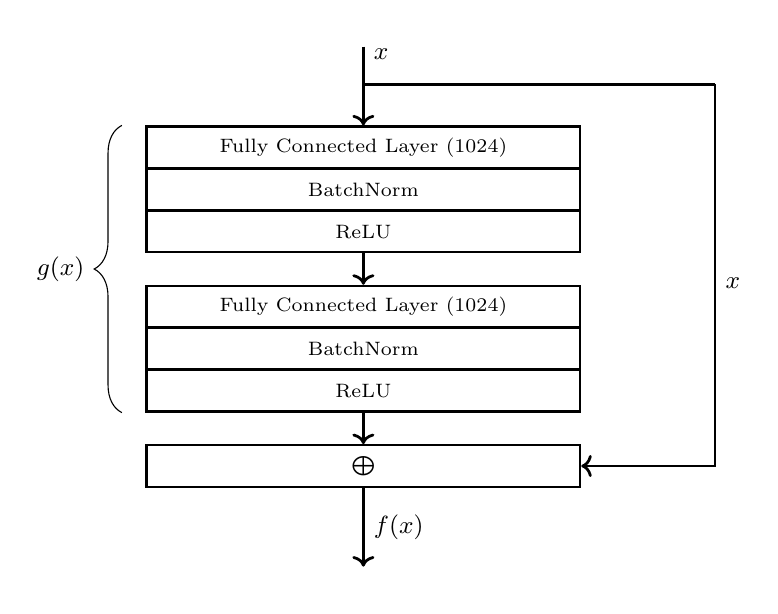
\begin{tikzpicture}
		[
		font=\scriptsize,
		block/.style ={rectangle, draw=black, thick, text width=15em, align=center, minimum height=1.5em}
		]
		\node[] (a) [block] {Fully Connected Layer (1024)};
		\node[below= -1.5\pgflinewidth of a] (a1) [block] {BatchNorm};
		\node[below= -1.5\pgflinewidth of a1] (b) [block] {ReLU};
		\node[below= 4mm of b] (c) [block] {Fully Connected Layer (1024)};
		\node[below= -1.5\pgflinewidth of c] (c1) [block] {BatchNorm};
		\node[below= -1.5\pgflinewidth of c1] (d) [block] {ReLU};
		\node[below= 4mm of d] (e) [block] {$\bigoplus$};
		\node[above=of a] (x) [] {};
		\draw[->, line width=1pt] (b.south) -- (c.north);
		\draw[->, line width=1pt] (d.south) -- (e.north);
		\draw[->, line width=1pt] (x) -- node [pos=0.1, right] {\small $x$} (a);
		\node[below=of e] (y) [] {};
		\draw[->, line width=1pt] (e) -- node [midway, right] {\small $f(x)$} (y);
		\node[above=.4 of a] (z) [] {};
		\node[right=12em of z] (h) [] {};
		\draw[line width=1pt] (z.center) -- (h.center);
		\draw[->, line width=1pt] (h.center) |- node [pos=.26,right] {\small $x$} (e.east);
		\draw [decorate, decoration={brace, amplitude=10pt}] ([xshift=-0.3cm]d.south west)-- ([xshift=-0.3cm]a.north west) node [black,midway, left, xshift=-10pt]{\small $g(x)$};
	\end{tikzpicture}
}
	\label{fig:residual-block}
\end{figure}
	\end{frame}

	\begin{frame}{Simplified Model of ResNets}
		content...
	\end{frame}

	\begin{frame}{Discrete Stationary Action}
		content...
	\end{frame}
	
	\begin{frame}{Continuous Stationary Action}
		content...
	\end{frame}

	\begin{frame}{Hamiltonian Formulation}
		content...
	\end{frame}

	\begin{frame}{Geodesic Shooting}
		content...
	\end{frame}

	\begin{frame}{Problem and Convergence Overview}
		\begin{figure}
	\makebox[\textwidth][c]{
		\centering
		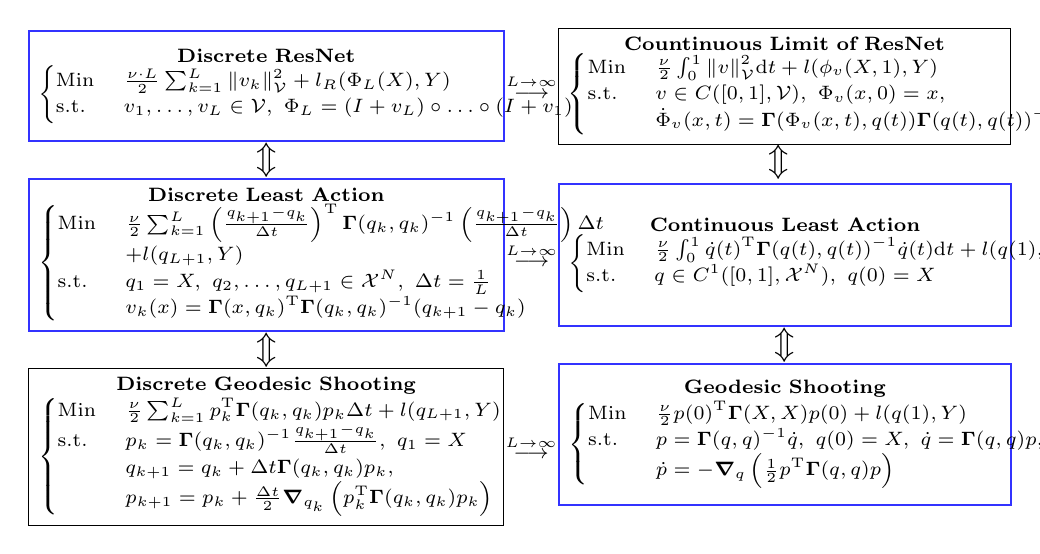
\begin{tikzpicture}[font=\scriptsize, align=center, node distance = 6mm and 6mm]
				\node[draw=blue!80,thick, above left, align=center, text width=58mm, minimum height=14mm] (a) {
					\textbf{Discrete ResNet}\\
					$\begin{cases}
						\text{Min~} & \frac{\nu \cdot L}{2} \sum_{k=1}^{L} \norm{v_k}_\cV^2
						+ l_R(\Phi_L(X), Y) \\
						\text{s.t.~} & v_1, \ldots, v_L \in \cV,\ \Phi_L = (I + v_L) \circ \ldots \circ (I + v_1)
					\end{cases}$};
				\node[right=of a, align=center,outer sep=-2em] (z1) {$\stackrel{L \rightarrow \infty}{\longrightarrow}$};
				\node[draw, right= of z1, align=center,text width=55mm, minimum height=14mm] (b) {
					\textbf{Countinuous Limit of ResNet}\\
					$\begin{cases}
						\text{Min~}& \frac{\nu}{2} \int_{0}^{1} \norm{v}_\mathcal{V}^2 \mathrm{d}t
						+ l(\phi_v(X, 1), Y)\\
						\text{s.t.~}& v \in C([0, 1], \mathcal{V}),\ \Phi_v(x, 0) = x,\\
						&\dot{\Phi}_v(x, t) = \mathbf{\Gamma}(\Phi_v(x, t), q(t)) \bGamma(q(t), q(t))^{-1} \dot{q}(t)
					\end{cases}$};
				\node[below= of a,outer sep=-2em] (z2) {\large{$\Updownarrow$}};
				\node[draw=blue!80, thick, below= of z2, align=center, text width=58mm, minimum height=18mm] (c) {
					\textbf{Discrete Least Action}\\
					$\begin{cases}
						\text{Min~} & \frac{\nu}{2} \sum_{k=1}^{L} \left(\frac{q_{k+1} - q_k}{\Delta t}\right)^\mathrm{T} \bGamma(q_k, q_k)^{-1} \left(\frac{q_{k+1} - q_k}{\Delta t}\right) \Delta t\\
						&+ l(q_{L+1}, Y) \\
						\text{s.t.~} & q_1 = X,\ q_2, \ldots, q_{L+1} \in \cX^N,\ \Delta t = \frac{1}{L}\\
						& v_k(x) = \bGamma(x, q_k)^\mathrm{T}\bGamma(q_k, q_k)^{-1} (q_{k+1} - q_k)
					\end{cases}$};
				\node[below= of b,outer sep=-2em] (z3) {\large{$\Updownarrow$} };
				\node[right=of c, align=center,outer sep=-2em] (z4) {$\stackrel{L \rightarrow \infty}{\longrightarrow}$};
				\node[draw=blue!80,thick, below= of z3, right=of z4, align=center, text width=55mm, minimum height=18mm] (d) {
					\textbf{Continuous Least Action}\\
					$\begin{cases}
					\text{Min~} & \frac{\nu}{2} \int_{0}^{1} \dot{q}(t)^\mathrm{T} \mathbf{\Gamma}(q(t), q(t))^{-1}  \dot{q}(t) \mathrm{d}t + l(q(1), Y)\\
					\text{s.t.~} & q \in C^1([0,1], \cX^N),\ q(0) = X
					\end{cases}$};
				\node[below= of d,outer sep=-2em] (z5) {\large{$\Updownarrow$}};
				\node[draw=blue!80,thick, below= of z5, align=center, text width=55mm, minimum height=18mm] (e) {
					\textbf{Geodesic Shooting}\\
					$\begin{cases}
						\text{Min~} & \frac{\nu}{2} p(0)^\T \bGamma(X, X)p(0) + l(q(1), Y)\\
						\text{s.t.~} & 	p = \bGamma(q, q)^{-1}\dot{q},\ q(0) = X,\ \dot{q} = \bGamma(q, q) p,\\
						&\dot{p} = -\grad_q \left(\frac{1}{2} p^\mathrm{T} \bGamma(q, q) p\right)
					\end{cases}$};
				\node[below= of c,outer sep=-2em] (z6) {\large{$\Updownarrow$}};
				\node[draw, below= of z6, align=center, text width=58mm, minimum height=18mm] (f) {
					\textbf{Discrete Geodesic Shooting}\\
					$\begin{cases}
					\text{Min~} & \frac{\nu}{2} \sum_{k=1}^L p_k^\T \bGamma(q_k, q_k) p_k \Delta t + l(q_{L+1}, Y)\\
					\text{s.t.~} & p_k = \bGamma(q_k, q_k)^{-1} \frac{q_{k+1} - q_k}{\Delta t},\ q_1 = X \\
					& q_{k+1} = q_k + \Delta t \bGamma(q_k, q_k) p_k,\\
					& p_{k+1} = p_k + \frac{\Delta t}{2} \grad_{q_k} \left(p_k^\T \bGamma(q_k, q_k) p_k\right)
					\end{cases}$};
				\node[right=of f, align=center,outer sep=-2em] (z7) {$\stackrel{L \rightarrow \infty}{\longrightarrow}$};
		\end{tikzpicture}
	}
	\label{fig:convergence}
\end{figure}
	\end{frame}

	\begin{frame}{Algorithm}
	\end{frame}

	\begin{frame}{Experimental Results}
	\end{frame}


	\begin{frame}
		\bibliography{bibliography}
		\bibliographystyle{plainnat}
	\end{frame}
\end{document}